\documentclass[12pt]{article}

\usepackage[english]{babel}
\usepackage[margin=0.8in]{geometry}

% Math/Greek packages
\usepackage{amssymb,amsmath,amsthm, mathtools} 
\usepackage{algorithm, algorithmic}
\usepackage{upgreek, siunitx}
\usepackage{setspace}

% Graphics/Presentation packages
\usepackage{multirow}
\usepackage{graphicx}
\usepackage{cancel}
\usepackage{tabulary, enumitem, array}
\usepackage{xparse,mleftright,tikz}
\usepackage{physics}

% Misc packages
\usepackage{fancyhdr}


\usepackage[export]{adjustbox}

\usepackage{esint}

\sisetup{locale=US,group-separator = {,}}
\usepackage[colorlinks=true, allcolors=blue]{hyperref}


% Box function - update this as more sophisticated solutions are found
\newcommand\mybox[2][]{\tikz[overlay]\node[fill=blue!20,inner sep=2pt, anchor=text, rectangle, rounded corners=1mm,#1] {#2};\phantom{#2}}
\renewcommand{\arraystretch}{1.2}

% General macro declarations


\makeatletter
\let\oldabs\abs
\def\abs{\@ifstar{\oldabs}{\oldabs*}}
%
\let\oldnorm\norm
\def\norm{\@ifstar{\oldnorm}{\oldnorm*}}
\makeatother

\begin{document}

\title{PHSX 491: HW03}
\author{William Jardee}
\maketitle

\section*{Question 1}

\[\Phi(x,y) = bxy\]

\begin{enumerate}[label=\alph*)]
\item Find the components of the gradient for $\Phi$ in Cartesian coordinates $\partial_\mu \Phi$.

$\partial_\mu \Phi \rightarrow \left[\pdv{x} \hat{x} + \pdv{y}\hat{y}\right] \Phi= by\hat{x} +bx\hat{y}$
\[\boxed{\mqty{A_x = by \\ A_y = bx}}\]

\item Convert $\Phi$ to the polar coordinates $(r,\theta)$.

We can use the relationships: $x = r\cos(\theta)$ and $y = r\sin(\theta)$
\[\boxed{\Phi(r, \theta) = br^2 \cos(\theta)\sin(\theta)}\]

\item Calculate $\partial_r \Phi$ and $\partial_\theta \Phi$.

To this one right, I figured out that we have to use the gradient in polar coordinates:
\[\partial_\mu \rightarrow \pdv{r} \hat{r} + \frac{1}{r}\pdv{\theta}\hat{\theta}\]
Using this, and grouping terms, we get:
\[\boxed{\mqty{A_r = 2br\cos(\theta)\sin(\theta) \\ A_\theta = br^2 [\cos[2](\theta) - \sin[2](\theta)]}}\]

\item If we transform the gradient from Cartesian to polar coordinates, do we get the components found above? That is, do the above components transform like a covector?

So, I see two ways to do this question. I will just go about both of them and hopefully satisfy that the gradient does transform like a covector:

$by \hat{x} + bx \hat{y} = br\sin(\theta)\hat{x} + br\cos(\theta)\hat{y}$

using the fact that $\hat{x} = \cos(\theta)\hat{r} - \sin(\theta)\hat{\theta}$ and $\hat{y} = \sin(\theta)\hat{r} + \cos(\theta)\hat{\theta}$:

\begin{flalign*}
by \hat{x} + bx \hat{y}& = br\sin(\theta)[\cos(\theta)\hat{r} - \sin(\theta)\hat{\theta}] + br\cos(\theta)[\sin(\theta)\hat{r} + \cos(\theta)\hat{\theta}]& \\ 
& = 2br\cos(\theta)\sin(\theta)\hat{r} + br[-\sin[2](\theta) + \cos[2](\theta)]\hat{\theta}&
\end{flalign*}

So, by this method, it works. Now, let's do it with a more sophisticated approach:

\[A_{\mu^\prime} = \pdv{x^\mu}{x^{\mu^\prime}}A_\mu\]

$A_r = \pdv{x}{r}A_x + \pdv{y}{r}A_y = \cos(\theta)br\sin(\theta) + \sin(\theta)br\cos(\theta) = 2br\cos(\theta)\sin(\theta)$

$A_\theta = \pdv{x}{\theta}A_x + \pdv{y}{\theta}A_y = -\sin(\theta)br\sin(\theta) + \cos(\theta)br\cos(\theta) = br[\cos[2](\theta) - \sin[2](\theta)]$

\[\boxed{\mqty{A_r = 2br\cos(\theta)\sin(\theta) \\ A_\theta = br^2 [\cos[2](\theta) - \sin[2](\theta)]}}\]

So, it looks that the gradient does transform like a covector! ({\sl Phew!})


\item Consider the points $P=(1,1)$, $Q=(-2,-1)$, and $R = (1,-3)$. How do the collection of surfaces described by the gradient behave at these points?

\begin{center}
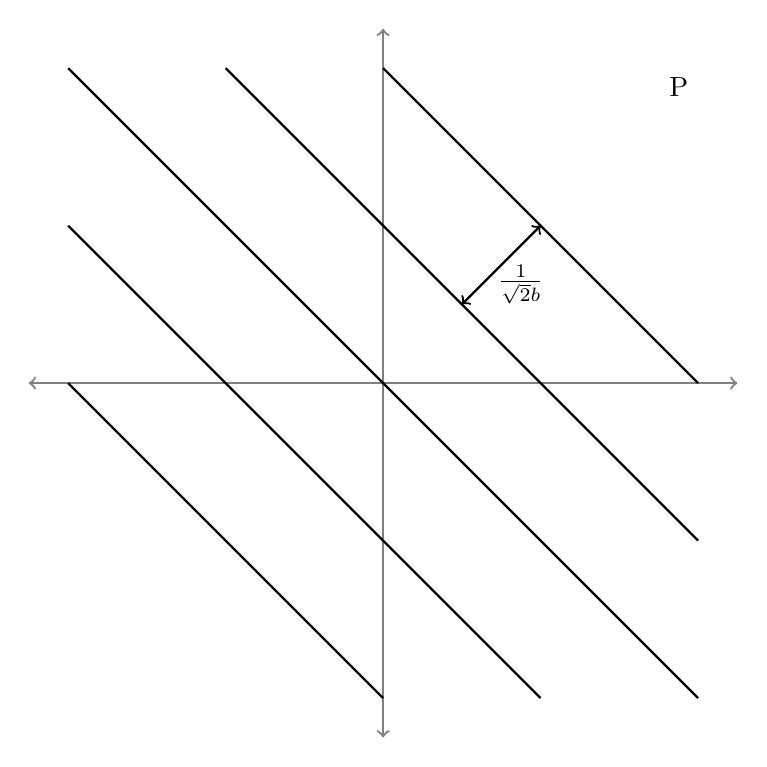
\begin{tikzpicture}
\draw[thick,gray,<->] (-4.5,0) -- (4.5,0);
\draw[thick,gray,<->] (0,-4.5) -- (0,4.5);
\foreach \x in {0, 1,2}
	\draw[thick, -]	 (-4+\x*2 ,4) -- (4,-4+\x*2 );
\foreach \x in {1,2}
	\draw[thick, -]	 (-4 ,4-\x*2) -- (4-\x*2,-4);
\draw[thick,<->] (1,1) -- (2,2);
\draw (1.75,1.25) node[anchor = center] {$\frac{1}{\sqrt{2}b}$};
\draw (4,4) node[anchor=north east] {P};
\end{tikzpicture}

\resizebox{0.45\textwidth}{!}
{
\begin{tikzpicture}
\draw[thick,gray,<->] (-4.5,0) -- (4.5,0);
\draw[thick,gray,<->] (0,-4.5) -- (0,4.5);
\foreach \x in {-1,0,1}
	\draw[thick, -] (4,-2-2*\x) -- (-4,2-2*\x);
\draw[thick,<->] (0,0) -- (0.8,1.6);
\draw (0.8,0.8) node[anchor = center] {$\frac{1}{\sqrt{5}b}$};
\draw (4,4) node[anchor=north east] {Q};
\end{tikzpicture}
}
\resizebox{0.45\textwidth}{!}
{
\begin{tikzpicture}
\draw[thick,gray,<->] (-4.5,0) -- (4.5,0);
\draw[thick,gray,<->] (0,-4.5) -- (0,4.5);
\foreach \x in {-1,0,1}
	\draw[thick, -] (1+1/3-2*\x,4) -- (-1-1/3-2*\x, -4);
\draw[thick,<->] (0,0) -- (-3*0.6,1*0.6);
\draw (-0.8,0.8) node[anchor = center] {$\frac{1}{\sqrt{10}b}$};
\draw (4,4) node[anchor=north east] {R};
\end{tikzpicture}
}
\end{center}

I tried to do the graphing in \LaTeX, so it is a bit scuffed. However, I think it kinda worked. 

For point P: The gradient turns into the set $A_x = b$, $A_y = b$. So, the covector will be perpendicular to this, with a slope $-1$.

For point Q: The gradient turns into the set $A_x = -b$, $A_y = -2b$. So, the covector will have the slope $-1/2$.

For point R: The gradient turns into the set $A_x = -3b$, $A_y = b$. So, the covector will have the slope $3$.


\begin{table}[!hb]
\centering
\begin{tabular}{llrccc}
\multirow{4}{*}{\rotatebox{90}{increasing}} &                                                & Point                  & $\partial_\mu$ & Slope          & Density      \\ \cline{3-6} 
                                                               & \multirow{3}{*}{$\bigg\downarrow$} & \multicolumn{1}{r|}{P} & $[b,b]$        & $-1$           & $\sqrt{2}b$  \\
                                                               &                                                & \multicolumn{1}{r|}{Q} & $[-b,-2b]$     & $-\frac{1}{2}$ & $\sqrt{5}b$  \\
                                                               &                                                & \multicolumn{1}{r|}{R} & $[-3b,b]$      & $3$            & $\sqrt{10}b$
\end{tabular}
\end{table}

\end{enumerate}


\end{document}
